\documentclass{article}
\usepackage{tabularx}
\usepackage{amsmath}
\usepackage{graphicx}
\usepackage[margin=2cm]{geometry}
\usepackage{cite}
\usepackage[final]{hyperref}
\usepackage{listings}
\usepackage{here}
\hypersetup{
	colorlinks=true,
	linkcolor=blue,
	citecolor=blue,
	filecolor=magenta,
	urlcolor=blue         
}

\begin{document}

\title{TP07\\Generate a fractal with Vulkan}
\author{Robin Faury}
\date{02/12/20}
\maketitle

\begin{abstract}
	In this practical work, we will reach the last step for fractal generation using Vulkan. This is also the end of practical for the mark. Other TP will explore advance GPU features.
\end{abstract}

\section{Dispatch}
We saw in the last practical the command dispatch can take three variable corresponding to x, y and z. Modify the call to pass the width and the height insted of the bufferSize. The push constant command must take two uint32\_t and the shader should get the two parameters.

\begin{lstlisting}
	layout(push_constant) uniform ImageSize {
		uint width;
		uint height;
	} imageSize;
\end{lstlisting}

You can now have an int as 'x' and an int as 'y' on your shader. You can apply the same critical path developed in the TP01 to generate the Mandelbrot set.

\begin{figure}[H]
	\centering
	
\includegraphics[scale=0.2]{figures/Mandelbrot.png}
	\caption{Mandelbrot set computed on GPU}
\end{figure}

\section{Profiling}
It's time to compare the computation speed between the CPU multithreaded and the GPU. Use the std::chrono object from the STL to profile the sendData, the computation and the getData.

\section{Work Groupe}
If your image has a size of 2048x2048, you run our shader using the dispatch function like this:
\begin{lstlisting}
	vkCmdDispatch(commandBuffer, 2048, 2048, 1);
\end{lstlisting}
That means you want to run 2048x2048 work group. Each work group will run one compute shader invocation. Take a look on the VkPhysicalDeviceProperties object to check if the maxComputeWorkGroupeSize allow you to run 2048 work group on the 'x' and 'y' dimension. Save the value of maxComputeWorkGroupInvocations too. We will try to dispatch less work group with more compute shader invocations. Just after the shader version in your GLSL code, add the layout of your work group:

\begin{lstlisting}
	layout(local_size_x = X, local_size_y = Y, local_size_z = 1) in;
\end{lstlisting}

The X and Y value are 1 by default. You can choose any combinaisons but keep in mind that $local\_size\_x * local\_size\_y * local\_size\_z <= maxComputeWorkGroupInvocations$. On your shader the image coordinate can be computed using gl\_WorkGroupID * gl\_WorkGroupSize + gl\_LocalInvocationID instead of gl\_GlobalInvocationID.

\begin{figure}[h]
	\centering
	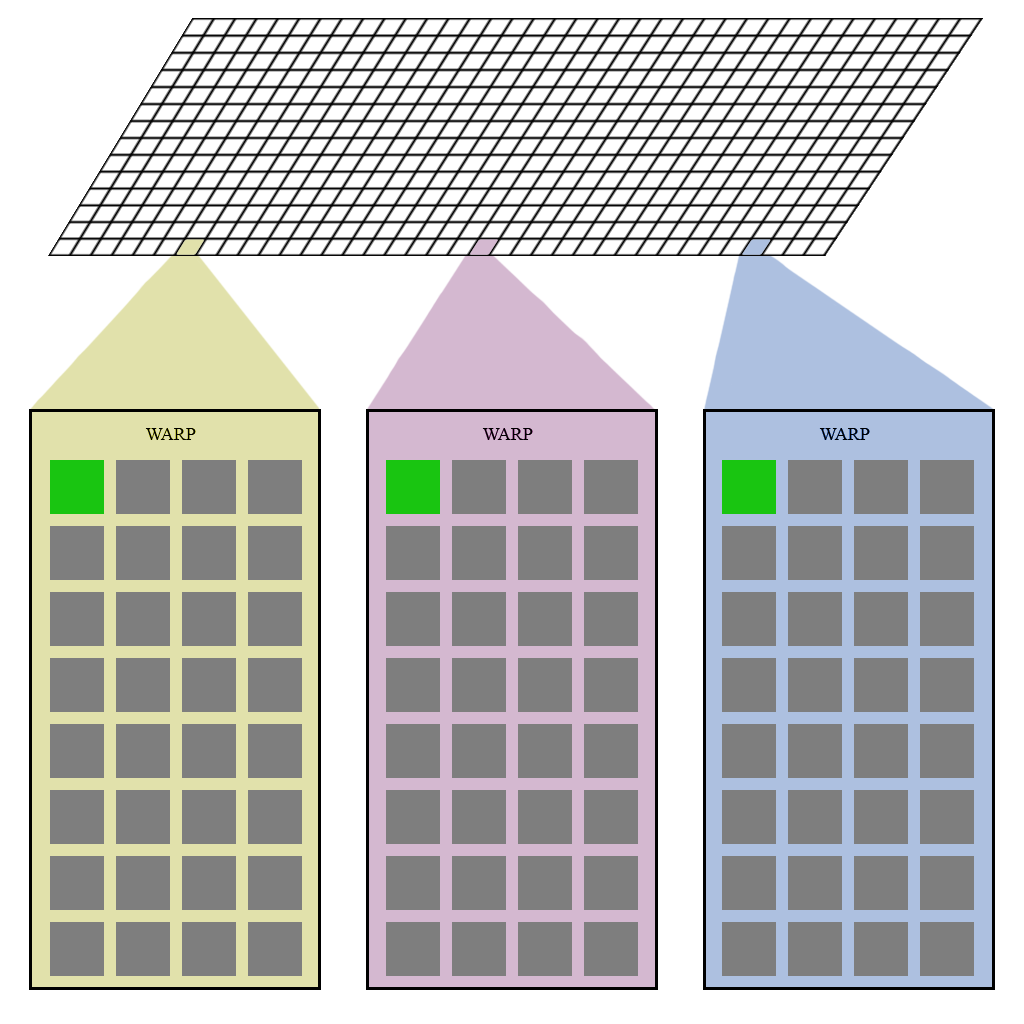
\includegraphics[scale=0.2]{figures/work_groupe_1.png}
	\caption{3 pixels processed with 1 shader invocation from 3 work groupes}
\end{figure}

\begin{figure}[h]
	\centering
	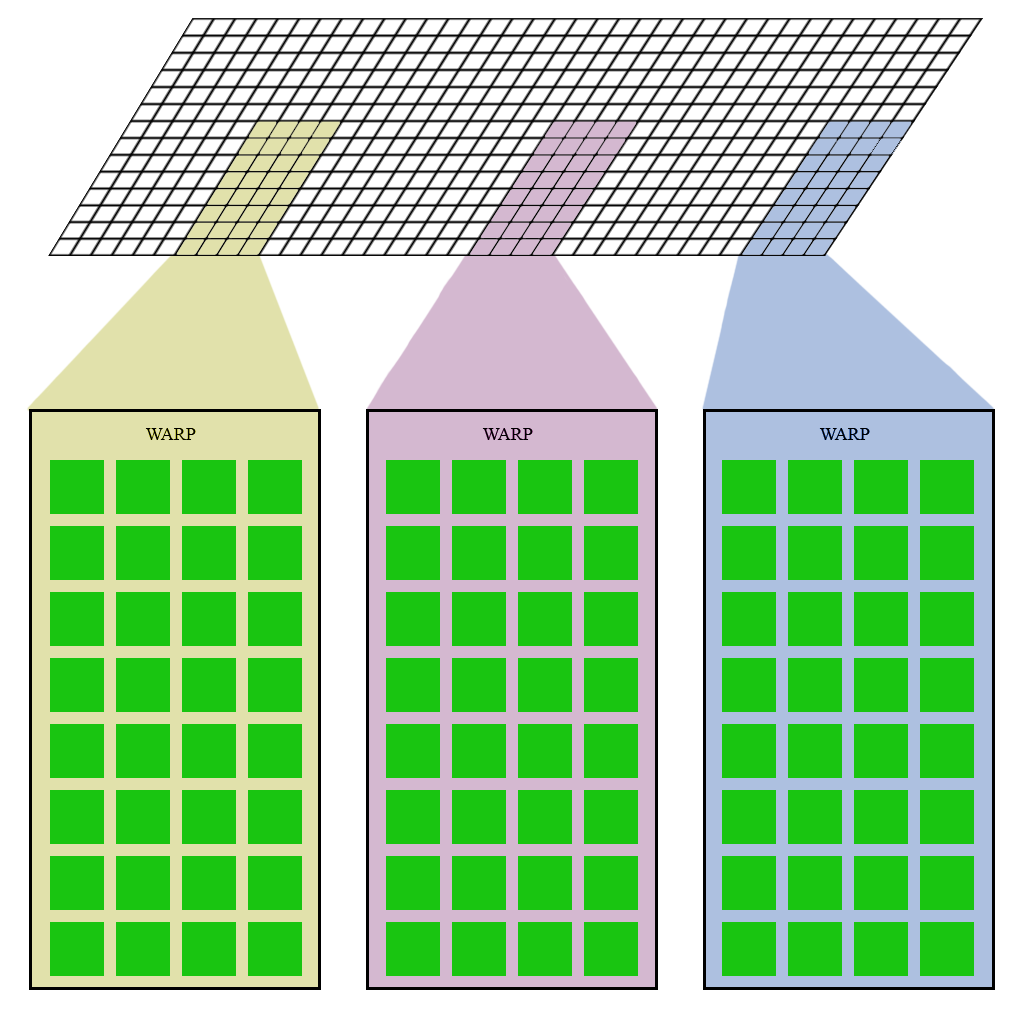
\includegraphics[scale=0.2]{figures/work_groupe_0.png}
	\caption{96 pixels processed with 32 shader invocations from 3 work groupes}
\end{figure}

\end{document}